

\chapter{ شبکه‌های مبتنی بر داده‌های نام‌گذاری شده}
در این فصل به معرفی شبکه‌های مبتنی بر داده‌های نام‌گذاری شده می‌پردازیم که ازین به بعد به اختصار آن را NDN(Named Data Networks) می‌نامیم.  در ابتدا به بررسی ایرادات شبکه‌های مبتنی بر IP که امروزه به طور گسترده استفاده می‌شوند و در حقیقت زیرساخت شبکه‌های امروزی را تشکیل می‌دهند می‌پردازیم و لزوم روی کار آمدن یک سیستم جدید را نشان می‌دهیم. در ادامه توضیحات مفصلی راجع به شبکه‌های NDN و چگونگی کارکرد آن‌ها داده می‌شود. در مرحله بعد، راجع به این‌که چگونه شبکه‌های NDN ایرادات شبکه‌های قبلی را مرتفع می‌کند و مزایای استفاده از آن بحث می‌شود. 

\section{زمینه و چشم‌انداز}
در دنیای امروز، 

\section{پایه‌های معماری}
در طراحی معماری شبکه‌های NDN، ۶ پایه درنظر گرفته شده است. ۳ مورد اول پایه‌هایی هستند که از موفقیت سیستم مبتنی بر IP امروزی ناشی می‌شوند و سه مورد آخر ناشی از مسائلی است که گسترش شبکه‌های امروزی آن‌ها را به صورت تجربی اثبات کرده‌اند. 
\begin{itemize}
\item{
\textit{معماری ساعت‌شنی}
 چیزی است که طراحی اینترنت امروزی را منحصربه‌فرد و قدرت‌مند می‌کند. محوریت این معماری لایه جهانی IP  است که کمینه عملکرد را برای ارتباطات فراهم کرده است. همچنین این لایه دلیل رشد بدون محدودیت شبکه‌های امروزی است چرا که لایه‌های بالاتر و پایین‌تر مستقل از اینکه چه اتفاقی در لایه IP  رخ می‌دهد می‌تواند بدون محدودیت گسترش پیدا کنند. همان‌طور که در شکل
~\ref{fig:hourglass}
  مشاهده می‌شود، شبکه‌های NDN هم همین معماری ساعت شنی را استفاده کرده است. 


\begin{figure}[H]
\centering
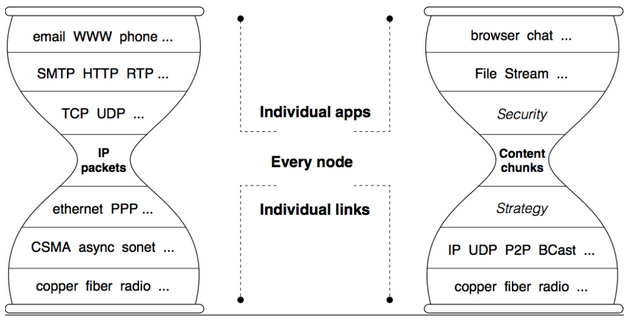
\includegraphics[scale=0.55]{./resources/figures/3_hourglass.png}
\caption{معماری ساعت‌شنی در شبکه‌‌ی اینترنت امروزی و شبکه‌ی NDN}
\label{fig:hourglass}
\end{figure}


%{\begin{figure}[t] \centering \includegraphics[width=#1cm]{resources/figures/#3.png} \caption{#2.} \label{fig:#3} \end{figure}}


} 

\item{
\textit{امنیت}
 یکی از ملزومات طراحی هر معماری‌ای است. امنیت در شبکه‌های امروزی، مسئله‌ای است که بعد از طراحی معماری به آن پرداخته شده است و در واقع در لایه‌های بالاتر و پایین‌تر از لایه شبکه به مسئله امنیت پرداخته شده و در محیط خطرناک اینترنت امروزی، امنیت مورد نیاز را تامین نمی‌کند. امنیت در شبکه‌های NDN یک مسئله پایه‌ای است و برخلاف شبکه‌های IP در همان لایه شبکه به آن پرداخته شده است و با امضا کردن محتوای بسته‌های داده این امنیت را در حد خوبی فراهم کرده است. 

}

\item{
\textit{روش انتها به انتها}
 که در شبکه‌های امروزی وجود دارد امکان مقابله در صورت بروز مشکل در شبکه  را فراهم می‌کند. اگر از روش انتها به انتها استفاده کنیم، در صورت از کار افتادن یکی از پیوندهای موجود در شبکه، از‌آنجایی که فقط به مقصد رسیدن بسته مهم است، مسیریاب می‌تواند بسته را از یک مسیر دیگر بفرستد و بسته در نهایت به مقصد خود می‌رسد ولی در صورتی که اگر از روش نقطه به نقطه استفاده شده باشد، در صورت بروز چنین رخدادی، بسته در میانه‌ی راه رها می‌شود. این رویه در شبکه‌های NDN هم وجود دارد. 
}

\item{
\textit{ترافیک شبکه}
باید به نحوی باشد که بتواند خودش را با تغییرات تطبیق دهد. جریان معتدل داده‌ها در داخل شبکه برای داشتن یک شبکه پایدار ضروری است. در سیستم مبتنی بر IP ، چون امکان به وجود آمدن حلقه در رسیدن بسته‌ها به مقصد وجود دارد، پروتکل‌های لایه انتقال هستند که در مقابل رویداد چنین وقایعی ارتقا داده شده‌اند. ولی در شبکه‌‌های NDN، در همان لایه شبکه مکانیزمی برای مقابله با به وجود آمدن حلقه در نظر گرفته شده است. 
}
\item{
\textit{جدا بودن دامنه مسیریابی و ارسال}
یکی از مسائلی است که ثابت شده برای توسعه اینترنت امری ضروری است. فایده این کار این است که سیستم ارسال می‌تواند به کار خود ادامه دهد درحالیکه سیستم مسیریابی به صورت مستقل خودش را با تغییرات شبکه تطبیق می‌دهد.  معماری حاکم بر NDN هم همین رویه را پیش‌رو گرفته و امکان مستقل کار کردن این دو دامنه را فراهم کرده است. 
}

\item{
\textit{ معماری باید انتخاب کاربر و رقابت را در مواقع امکان‌پذیر فراهم کند }
هرچند که این فاکتور، در طراحی معماری اصلی اینترنت جایگاهی نداشته است، ولی گسترش شبکه‌ها این قضیه را اثبات کرده است که معماری نباید نقش خنثی‌ای داشته باشد. معماری NDN تلاش آگاهانه‌ای در جهت قدرتمند کردن کاربران نهایی و همچنین به وجود آمدن رقابت کرده است. 
}

\end{itemize}

\section{معماری NDN}
مشابه شبکه‌های مبتنی بر IP، محوریت معماری شبکه‌های NDN  نیز همان میانه ساعت شنی ذکر شده در قسمت قبل است. ولی در این شبکه‌ها از داده‌‌های نام‌گذاری شده به جای آدرس‌های IP استفاده می‌‌شود. این تغییر علی‌رغم سادگی‌اش، موجب به وجود آمدن تفاوت‌های زیادی بین عملکرد این شبکه‌ها در رساندن بسته‌ها با شبکه‌های پیشین که مبتنی بر IP بودند، شده است.  در این بخش ابتدا یک توضیح مختصر راجع به مفاهیم کلی در شبکه‌های NDN داده می‌شود و سپس راجع به هر عنصر و هم‌چنین نقش آن در معماری کلی به تفضیل صحبت می‌شود. \\

\begin{figure}[H]
\centering
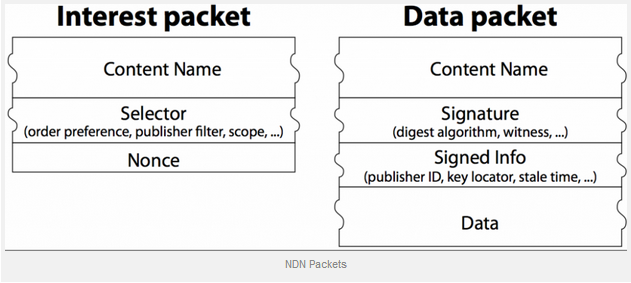
\includegraphics[scale=0.75]{./resources/figures/3_NDNpackets.png}
\caption{بسته‌ها در معماری NDN}
\label{fig:packets}
\end{figure}

\begin{figure}[H]
\centering
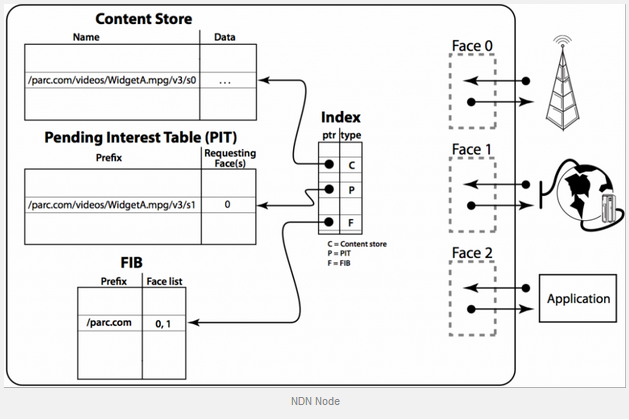
\includegraphics[scale=0.75]{./resources/figures/3_NDNnode.png}
\caption{ساختار یک مسیریاب در شبکه‌های مبتنی بر داده‌ی نام‌گذاری‌شده}
\label{fig:node}
\end{figure}



ارتباطات در شبکه‌های NDN بر پایه درخواست یک مشتری
\
 آغاز می‌شود. مشتری برای اینکه به داده‌ای دسترسی پیدا کند، یک بسته از نوع درخواست می‌فرستد که شامل یک نام است که ماهیت داده مورد نظر را مشخص می‌کند (شکل
‍‍‍‍~\ref{fig:packets}
). مسیریاب واسطی که این بسته از آن رسیده است را به خاطر می‌سپارد و بعد این بسته را بر پایه داده‌های \مهم{جدول اطلاعات ارسال}\زیرنوشت{Forwarding Informaion Base} (FIB) بر روی واسط درست ارسال می‌کند. این جدول به وسیله نتایج حاصل از کارکرد پروتکل مسیریابی به روزرسانی می‌شود. وقتی که بسته درخواست به گره‌ای رسید که حاوی اطلاعات موردنظر بود، یک بسته \textbf{داده} فرستاده می‌شود. که شامل نام و محتوایات داده است که به وسیله گره ارسال کننده اطلاعات امضا شده‌اند. مسیری که توسط بسته داده طی می‌شود تا به دست مشتری برسد، دقیقا برعکس مسیری است که بسته درخواست طی کرده است. لازم به ذکر است که هیچ‌کدام از بسته‌‌های درخواست و یا داده شامل هیچ آدرس میزبان و یا واسطی نظیر آنچه در IP  داریم، نیستند. بسته‌های درخواست براساس نام‌ای که در آن‌ها ذکر شده است، به سمت مقصد خود روانه می‌شوند و بسته‌های داده هم بر اساس اطلاعات نگه‌داری شده در هر گره بین راه حرکت می‌کنند تا به دست مشتری برسند. (‌شکل
~\ref{fig:node}
) \\
مسیریاب‌ها تمام درخواست‌‌های که منتظرند تا بسته داده آن‌ها برسد را در جدولی به نام \textbf{جدول درخواست‌‌های معلق} ذخیره‌ می‌کنند. وقتی که درخواست‌‌‌های متعددی برای یک داده به یک مسیریاب می‌رسد، فقط اولین درخواست به سمت منبع داده مورد نظر ارسال می‌شود. هر سطر جدول PIT شامل یک نام و همچنین تمام واسط‌‌هایی است که حداقل یک بسته درخواست برای این داده از طریق آن‌ها دریافت شده است. وقتی که یک بسته داده به مسیریاب می‌رسد، مسیریاب سطر مربوطه را از جدول ذخیره‌شده بازیابی می‌کند و بسته داده را به تمام واسط‌هایی که برای این داده ثبت شده بودند، ارسال می‌کند. سپس سطر مربوطه را از جدول PIT  حذف می‌کند و در ادامه، بسته داده را در \textbf{بانک داده} خود ذخیره‌سازی می‌کند. از آنجایی که یک بسته داده در شبکه‌های NDN مستقل از آنکه از کجا آمده و به کجا می‌رود، بامعنا است، مسیریاب‌ها می‌توانند آن‌ها را ذخیره کنند تا در موارد آینده که درخواست این داده به آن‌ها می‌رسد، به این درخواست پاسخ بگویند. 




\subsection{اسامی}
طراحی شبکه‌های NDN بر پایه‌ی نام‌گذاری‌های سلسله‌مراتبی و ساخت‌یافته‌ی داده‌ها است. برای مثال یک فیلم که شرکت سازنده‌ی آن PARC است، می‌تواند نام /parc/videos/WidgetA.mpg را داشته باشد. علامت / مشخص‌کننده مرز بین مولفه‌ها است و جزئی از نام محسوب نمی‌شود. این ساختار سلسله‌مراتبی به برنامه‌های این امکان را می‌دهد که روابط بین داده‌های مختلف را نمایش دهند. برای مثال، نام بخش ۳ از نسخه ۱ این فیلم می‌تواند /parc/videos/WidgetA.mpg/1/3 باشد. این ساختار همچنین باعث می‌شود که مسیریابی مقیاس‌پذیر شود. هرچند به صورت تئوری ممکن است که مسیریابی بر اساس نام‌های تخت (غیر سلسله‌مراتبی) هم صورت پذیرد،

 ولی این ساختار سلسله‌مراتبی است که امکان تجمع را فراهم می‌کند که در مبحث مسیریابی امری ضروری است. 


\subsection{امنیت داده‌محور}
\subsection{مسیریابی و ارسال}
\subsection{ذخیره‌سازی}
\subsection{جدول درخواست‌های معلق}
\subsection{انتقال}